%%%%%%%%%%%%%%%%%%%%%%%%%%%%%%%%%%%%%%%%%%%%%%%%%%%%%%%%%%%%%%%%%%%%%
% LaTeX Template: Curriculum Vitae
%
% Source: http://www.howtotex.com/
% Feel free to distribute this template, but please keep the
% referal to HowToTeX.com.
% Date: July 2011
% 
%%%%%%%%%%%%%%%%%%%%%%%%%%%%%%%%%%%%%%%%%%%%%%%%%%%%%%%%%%%%%%%%%%%%%%
% How to use writeLaTeX: 
%
% You edit the source code here on the left, and the preview on the
% right shows you the result within a few seconds.
%
% Bookmark this page and share the URL with your co-authors. They can
% edit at the same time!
%
% You can upload figures, bibliographies, custom classes and
% styles using the files menu.
%
% If you're new to LaTeX, the wikibook is a great place to start:
% http://en.wikibooks.org/wiki/LaTeX
%
%%%%%%%%%%%%%%%%%%%%%%%%%%%%%%%%%%%%%%%%%%%%%%%%%%%%%%%%%%%%%%%%%%%%%%
\documentclass[paper=a4,fontsize=11pt]{scrartcl} % KOMA-article class
							
\usepackage[english]{babel}
\usepackage[utf8x]{inputenc}
\usepackage[protrusion=true,expansion=true]{microtype}
\usepackage{amsmath,amsfonts,amsthm}     % Math packages
\usepackage{graphicx}                    % Enable pdflatex
\usepackage[svgnames]{xcolor}            % Colors by their 'svgnames'
\usepackage{geometry}
	\geometry{textheight=22cm, margin=2cm, a4paper}
\usepackage{url,fdsymbol,wasysym, comment}

\frenchspacing              % Better looking spacings after periods
\pagestyle{empty}           % No pagenumbers/headers/footers

%%% Custom sectioning (sectsty package)
%%% ------------------------------------------------------------
\usepackage{sectsty}

\sectionfont{%			            % Change font of \section command
	\usefont{OT1}{phv}{b}{n}%		% bch-b-n: CharterBT-Bold font
	\sectionrule{0pt}{0pt}{-5pt}{3pt}}

%%% Macros
%%% ------------------------------------------------------------
\newlength{\spacebox}
\settowidth{\spacebox}{8888888888}			% Box to align text
\newcommand{\sepspace}{\vspace*{0.8em}}		% Vertical space macro

\newcommand{\MyName}[1]{ % Name
		\Huge \usefont{OT1}{phv}{b}{n} \hfill #1
		\par \normalsize \normalfont}
		
\newcommand{\MySlogan}[1]{ % Slogan (optional)
		\large \usefont{OT1}{phv}{m}{n}\hfill \textit{#1}
		\par \normalsize \normalfont}

\newcommand{\NewPart}[1]{\section*{\uppercase{#1}}}

\newcommand{\PersonalEntry}[2]{
		\noindent\hangindent=2em\hangafter=0 % Indentation
		\parbox{\spacebox}{        % Box to align text
		\textit{#1}}		       % Entry name (birth, address, etc.)
		\hspace{1.5em} #2 \par}    % Entry value

\newcommand{\SkillsEntry}[2]{      % Same as \PersonalEntry
		\noindent\hangindent=2em\hangafter=0 % Indentation
		\parbox{\spacebox}{        % Box to align text
		\textit{#1}}			   % Entry name (birth, address, etc.)
		\hspace{1.5em} #2 \par}    % Entry value	
		
\newcommand{\EducationEntry}[4]{
		\noindent \textbf{#1} \hfill      % Study
		\colorbox{Black}{%
			\parbox{6em}{%
			\hfill\color{White}#2}} \par  % Duration
		\noindent \textit{#3} \par        % School
		\noindent\hangindent=2em\hangafter=0 \small #4 % Description
		\normalsize \par}

\newcommand{\WorkEntry}[4]{				  % Same as \EducationEntry
		\noindent \textbf{#1} \hfill      % Jobname
		\colorbox{Black}{\color{White}#2} \par  % Duration
		\noindent \textit{#3} \par              % Company
		\noindent\hangindent=2em\hangafter=0 \small #4 % Description
		\normalsize \par}

%%% Begin Document
%%% ------------------------------------------------------------
\begin{document}
% you can upload a photo and include it here...
%\begin{wrapfigure}{l}{0.5\textwidth}
\vspace*{-3em}
		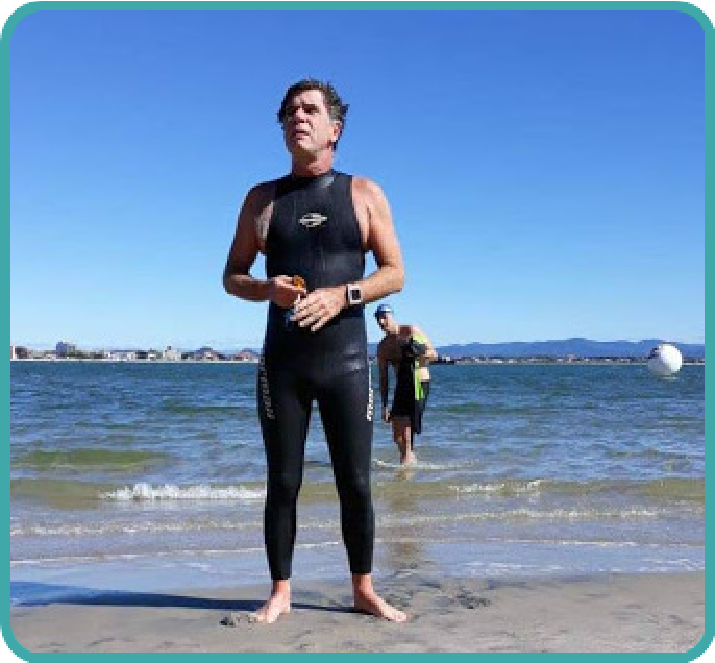
\includegraphics[width=0.35\textwidth]{figures/boas_bracadas.pdf}

%\end{wrapfigure}
\vspace{-1.5cm}
\MyName{Claudio Cesar de Sá}
\MySlogan{Curriculum Vitae}


\sepspace

%%% Personal details
%%% ------------------------------------------------------------
\NewPart{Self Presentation}{}

\begin{comment}
My name is Claudio and I am a retired professor of Computer Science in Brazil. So, it is not a conventional CV expected for you, once that I aiming news and different challenges in this new step of my life. It brings only highlights of my professional career, skills, and motivations. Everything in 2 pages \smiley{!}
\end{comment}

I am a retired professor of Computer Science in Brazil after teaching for more than 35 years courses like introduction to programming, symbolic artificial intelligence, mathematical logic, data structures and so much more. My experience involve mostly constraint programming, first-order logic, multi-paradigm programming and declarative languages (e.g. PROLOG, PICAT, Haskell, Minizinc, C/C++, Python, etc.). Now, I wish to start a new chapter of my career and I'm looking to shift towards helping solving industry-oriented real-world problems using the knowledge and expertise I acquired throughout my life. Please, check the note about my {\em availability} at the end of this CV.
\sepspace

%%% Personal details
%%% ------------------------------------------------------------
\NewPart{Personal details}{}

%\PersonalEntry{Birth}{May 10, 1959}
\PersonalEntry{Address}{Rua: Ex-Combatentes 125 -- Casa E3 -- 89.221-103 -- Joinville -- SC}
\PersonalEntry{Country}{Brazil}
\PersonalEntry{Phone}{(+55) 47 99245 1825}
\PersonalEntry{Mails}{\underline{\url{ccs1664@gmail.com}} -- \underline{\url{ccs1664@yahoo.com}}} \vspace{2mm}
\PersonalEntry{Site}{\underline{\url{https://claudiocesar.wordpress.com/}}}
\PersonalEntry{GitHub}{\underline{\url{https://github.com/claudiosa/}}}

%%% Education
%%% ------------------------------------------------------------
\NewPart{Education}{}


\EducationEntry{Post-doctorate Research (sabbatical year)}{2010 -- 2010}{Université d'Auvergne -- Clermont Ferrand -- Aurvegne -- France}{Grant support from  Coordination for the Improvement of Higher Education Personnel (CAPES -- Brazil). Subject: theoretical aspects of Constraint Programming.}
\sepspace

\EducationEntry{Doctor in Science}{1992--1997}{Aeronautics Institute of Technology (ITA) -- São José dos Campos -- SP -- Brazil}{Grant support from  Coordination for the Improvement of Higher Education Personnel (CAPES -- Brazil) and Federal University of Alagoas.} {Subject: Artificial Intelligence and Theory of Computation.}
\sepspace

\EducationEntry{Master in Science}{1982--1987}{Federal University of Paraíba (UFPb) -- Campina Grande -- PB -- Brazil}{Subject: Performance Network.}
\sepspace

\EducationEntry{Bachelor in Electrical Engineering}{1977-1981}{Santa Catarina State University (UDESC) -- Joinville -- SC -- Brazil}{Concentration: Electronic and Telecommunication}
%%% Work experience
%%% ------------------------------------------------------------
\NewPart{Work experience}%{I am describing here, only, the most recent jobs:}

\EducationEntry{WhatsTV}{2021 -- current}{\url{https://www.whatstv.com.br/}}{I had worked technical support for users of our product. As well as, I have been contact/tests with many Web technologies.}
\sepspace

\EducationEntry{Upwork}{2019 -- 2021}{\url{https://www.upwork.com/} -- Eventually,  on-demand.}{I had worked as a programmer in languages listed below, my profile is found in: \url{https://www.upwork.com/o/profiles/users/~019017be3783b12815/}. I am putting in hold on.}
\sepspace

\EducationEntry{Modal Institute (Instituto Modal)}{2020--2020}{Full-time -- \url{https://institutomodal.org.br/}}
{I worked for one month in a project with Prolog, consulting, training a team, and developer.}
\sepspace

\EducationEntry{Lecturer in Computer Science} {1986 -- 2019}{Many universities in Brazil as Computer Science professor}{During this period I taught and research in many universities in Brazil. The CNPq site brings a detailed CV about myself in: \underline{\url{http://lattes.cnpq.br/2946250323814779}}  This CV provided is strictly with an academic view. It is omitted due its size.}


%%% Skills
%%% ------------------------------------------------------------
\NewPart{Technical Skills}{}

\SkillsEntry{Operating System:} {\textsc{Windows}, \textsc{Linux}}

\SkillsEntry{Programming:} {\textsc{C++} ($\medstar\hspace{-1mm}\medstar$), \textsc{C} ($\medstar\hspace{-1mm}\medstar\hspace{-1mm}\medstar$), \textsc{Python} ($\medstar\hspace{-1mm}\medstar\hspace{-1mm}\medstar$), \textsc{Picat} ($\medstar\hspace{-1mm}\medstar\hspace{-1mm}\medstar\hspace{-1mm}\medstar\hspace{-1mm}\medstar$),  \textsc{Prolog} 
($\medstar\hspace{-1mm}\medstar\hspace{-1mm}\medstar\hspace{-1mm}\medstar\hspace{-1mm}\medstar$), ASP
($\medstar\hspace{-1mm}\medstar\hspace{-1mm}\medstar$), Haskell 
($\medstar\hspace{-1mm}\medstar\hspace{-1mm}\medstar$), BASH ($\medstar\hspace{-1mm}\medstar$) \\ where a $\medstar$: represents domain or fluency}

\SkillsEntry{Solvers:} {\textsc{Minizinc}, \textsc{OPL},
 \textsc{OR-TOOLS} and  \textsc{Answer Set Programming -- ASP}}

\SkillsEntry{Editors:} {\textsc{LibreOffice}, \LaTeX, \textsc{EMACS}}



%%% References
%%% ------------------------------------------------------------
\NewPart{Skills}{}

\begin{itemize}
\setlength\itemsep{-2mm}
\item Symbolic AI
\item Declarative Languages
\item Constraint Programming
\item Modelling in Combinatorial Problems

\end{itemize}
%%% ------------------------------------------------------------
\begin{comment}
\NewPart{Not my Cup of the Tea}{}

\begin{itemize}
\setlength\itemsep{-2mm}
\item Web developer
\item Front-end developer
\item Data-bank expert

\end{itemize}
\end{comment}

%%% 
%%% ------------------------------------------------------------
\NewPart{Languages}{}

\SkillsEntry{Languages:} {Portuguese (mother tongue)}
\SkillsEntry{}{English (fluent)}
\SkillsEntry{}{French (fluent -- except to write)}
\SkillsEntry{}{Spanish (good -- except to write)}


\NewPart{Availability}{}

Due my many reasons, at this moment, I am interested in a part-time job and remote. So, the consulting tasks has been more suitable for me. But, in the future, a changing country or city can be evaluated.

%%% References
%%% ------------------------------------------------------------
\NewPart{Leisures}{}

\SkillsEntry{Swimming:}{Active swimmer in open water competitions in Brazil -- level advanced in according my age!}
\sepspace

\SkillsEntry{My Youtube channel:} {\url{https://www.youtube.com/channel/UCdXNTAs1Sv7ARPr-TuViEUA}}

\end{document}



